%模板
\documentclass[10pt,a4paper,twoside]{book}

%文章标题设置
%中文名
\newcommand{\titleCN}{视觉SLAM 笔记}
%英文名
\newcommand{\titleEN}{Visual SLAM}
%版本号
\newcommand{\version}{V1.12.028$\,\,$(内测版)}

% ---------------------------- 宏包导入 ----------------------------  %
\usepackage[utf8]{inputenc}
\usepackage{ctex}
\usepackage{xeCJK}
\usepackage{cite}
\usepackage{makecell}
\usepackage{yhmath}
\usepackage{verbatim}
\usepackage{enumerate}%罗列专用宏包
\usepackage{graphicx}%插入图片的宏包
\usepackage{subfigure}
\let\widering\relax
\usepackage{newtxtext}
\usepackage{newtxmath}
\usepackage{bm}
\DeclareMathSizes{10}{10}{5.5}{5}
\usepackage{makeidx}%索引专用
\makeindex  %添加索引
\usepackage{fancyhdr}
%\usepackage{textcomp}%树叶图案在这个包里
%\usepackage{bbding}%很多漂亮的图案
\usepackage[dvipsnames, svgnames, x11names]{xcolor}%导入了所有颜色配置文件的宏包
\usepackage{geometry}%页边距调整
\geometry{left=2cm,right=2cm,bottom=2cm,top=2cm}
\usepackage{titletoc}%目录页的宏包
\usepackage{titlesec}%改变章节或标题的样式的宏包
\usepackage[bookmarks=true,colorlinks,linkcolor=black]{hyperref}
\usepackage{enumitem}
\usepackage{tcolorbox}%box宏包
\tcbuselibrary{most}
\usepackage{xcolor}
\usepackage{colortbl,booktabs}%第二个包定义了几个*rule  
\usepackage{multicol}
\usepackage{multirow}
\usepackage{tikz}
\usetikzlibrary{calc}
\usepackage{capt-of}
\usepackage{nomencl}%符号说明包
\usepackage{makecell}
\makenomenclature%制作符号说明
%\usepackage{longtable}
%\usepackage{polynom}% 除法竖式
\usetikzlibrary{shapes.geometric}
\usetikzlibrary{arrows,arrows.meta}
\pgfdeclarelayer{background}
\pgfdeclarelayer{foreground}
\pgfsetlayers{background,main,foreground}
%\usetikzlibrary{circuits.ee.IEC}
\usepackage{listings}
\usepackage{color}
\definecolor{dkgreen}{rgb}{0,0.6,0}
\definecolor{gray}{rgb}{0.5,0.5,0.5}
\definecolor{mauve}{rgb}{0.58,0,0.82}
\newfontfamily\monaco{Monaco}
\lstdefinestyle{C++}{                  %设置代码块
	basicstyle=\footnotesize\ttfamily,% 基本风格
	numbers=left,    % 行号
	numbersep=10pt,  % 行号间隔 
	tabsize=2,       % 缩进
	extendedchars=true, % 扩展符号?
	breaklines=true, % 自动换行
	language=C++,
    morekeywords={},
	keywordstyle=\color{blue},
	commentstyle=\color{dkgreen},
	stringstyle=\color{mauve},
    frame=tlrb,
    framerule=1pt,
    framesep=3pt,
    frameround = tttt,
    backgroundcolor=\color[RGB]{255,251,251},
    rulecolor=\color[RGB]{215,215,215},
	xleftmargin=19pt,% 竖线左边间距
	showspaces=false,% 空格字符加下划线
	showstringspaces=false,% 字符串中的空格加下划线
	showtabs=false,  % 字符串中的tab加下划线
}
\lstdefinestyle{bash}{                  %设置代码块
	basicstyle=\footnotesize\ttfamily,% 基本风格
	numbers=none,    % 行号
	tabsize=2,       % 缩进
	extendedchars=true, % 扩展符号?
	breaklines=true, % 自动换行
	language=bash,
    morekeywords={sudo,apt,git,wget,unzip},
	keywordstyle=\color{blue},
	commentstyle=\color{dkgreen},
	stringstyle=\color{mauve},
    frame=tlrb,
    framerule=1pt,
    framesep=3pt,
    frameround = tttt,
    backgroundcolor=\color[RGB]{255,251,251},
    rulecolor=\color[RGB]{215,215,215},
	xleftmargin=0pt,% 竖线左边间距
	showspaces=false,% 空格字符加下划线
	showstringspaces=false,% 字符串中的空格加下划线
	showtabs=false,  % 字符串中的tab加下划线
}
% ------------------------------------------------------------- %

% ---------------------------- 基本设置 ----------------------------  %
%字体设置
\setCJKmainfont[BoldFont={PingFangSC-Semibold}]{PingFangSC-Regular}

%调整间距(倍数)
\linespread{1.5}

%定义颜色
%定义某个颜色,对应颜色代号查表
\definecolor{titlepurple}{HTML}{5758BB}%一级标题(目前:蓝紫色)
\definecolor{titlepurpleb}{HTML}{3A006F}%二级标题(目前:深紫色)
\definecolor{titlepurplec}{HTML}{006266}%三级标题(目前:墨绿色)
\definecolor{tab1}{HTML}{9698ED}%表格1
\definecolor{tab2}{HTML}{DBDCFF}%表格2
\definecolor{dy0}{HTML}{EA7500}%小标题定义专用(目前:橙黄色)
\definecolor{dl}{HTML}{007500}%小标题定理专用(目前:深绿色)
\definecolor{inference}{HTML}{343300}%小标题推论专用(目前:墨绿色)
\definecolor{ex}{HTML}{7158e2}%小标题例专用(目前:紫色)
\definecolor{dy}{HTML}{BF0060}%夹杂在文本中的定义词的颜色1(目前:深红色)
\definecolor{dy2}{HTML}{FF0000}%夹杂在文本中的定义词的颜色2(目前:红紫色)
\definecolor{dya}{HTML}{FFFFFF}
\definecolor{超链接}{HTML}{0000C6}%含超链接的文字专用色(目前:蓝紫色)
\definecolor{文字底色}{HTML}{F8FF00}%强调的文字底色(目前:黄色)
\definecolor{eq}{HTML}{F0F0F0}
\definecolor{tl}{HTML}{D94600}

%章节或标题的样式
\titleformat{\chapter}{\bfseries\Huge\color{titlepurple}}{第\ \thechapter\ 章\ \quad}{0pt}{}
\titleformat{\section}{\bfseries\Large\color{titlepurpleb}}{\bfseries{\thesection}\quad  }{0pt}{}
\titleformat{\subsection}{\bfseries\large\color{titlepurplec}}{\bfseries{\thesubsection}\quad  }{0pt}{}
%\titlespacing{\subsection}{1.5em}{0.1em}{1em}[1em]
%格式如下:\titlespacing*{章节名称}{左间距}{(前)行间距}{(后)行间距}[右间距(一般都没用,填0.1em即可,但不能不填)]


%目录调整
\newcounter{mycontents}
\newcommand{\thecontents}{\refstepcounter{mycontents} \alph{mycontents}.}
%\titlecontents{标题名}[左间距]{标题格式}{标题标志}{无序号标题}{指引线与页码}[下间距]
\titlecontents{chapter}
[0cm]
{\bf \large \vspace{0.8em} }{\contentspush{第 \thecontentslabel\ 章 \hspace*{0.8em}}}{}{\titlerule*[0.5pc]{$\cdot$}\contentspage}
\titlecontents{section}[1.7cm]{\bf  \vspace{0.5em} }{\contentslabel{2.4em}}{\hspace*{-2.5em} \thecontents \hspace*{0.8em}}{\titlerule*[0.5pc]{$\cdot$}\contentspage}
\titlecontents{subsection}[2.5cm]{\small \vspace{0.2em} }{\contentslabel{3em}}{}{\titlerule*[0.5pc]{$\cdot$}\contentspage}

%自定义页眉页脚---------------
\pagestyle{fancy}
\renewcommand{\chaptermark}[1]{\markboth{\;第\ \thechapter\ 章\quad#1\;}{}}
\renewcommand{\sectionmark}[1]{\markright{\;\thesection\ #1\;}}
\fancyhf{}
%\fancyfoot[C]{\bfseries\thepage}
\fancyhead[LO]{\small\CJKfamily{song}\rightmark}
\fancyhead[RE]{\small\CJKfamily{song}\leftmark}
\fancyhead[RO,LE]{\;\thepage\;}
\fancyfoot[RO,LE]{\footnotesize\CJKfamily{heilight}{\titleCN}}
\fancyfoot[RE,LO]{\footnotesize\CJKfamily{heilight}\titleEN}
\renewcommand{\headrulewidth}{0.4pt} % 注意不用\setlength
%\renewcommand{\footrulewidth}{0pt}
\fancyheadoffset[LE,RO]{0cm}
\fancyfootoffset[LE,RO]{0cm}
% 注意不用\setlength
%\renewcommand{\footrulewidth}{0pt}
% ------------------------------------------------------------- %


% ---------------------------- 定义环境 ----------------------------  %

%定义计数器
\newcounter{theorem}[chapter]
\newcounter{defination}[chapter]
\newcounter{example}[chapter]
\newcounter{inference}[chapter]
\newcounter{examples}[chapter]
\newcounter{tl}[chapter]
\newcounter{lemma}[chapter]
\newcounter{F}[section]
\newcounter{G}[section]
\newcounter{H}[section]
\renewcommand{\thetheorem}{{ 定理} \textbf{\thechapter.\arabic{theorem}}}
\renewcommand{\thedefination}{{ 定义} \textbf{\thechapter.\arabic{defination}}}
\renewcommand{\theexample}{{ 题型} \textbf{\thechapter.\arabic{example}}}
\renewcommand{\theinference}{{ 方法} \textbf{\thechapter.\arabic{inference}}}
\renewcommand{\theexamples}{{ 例}  \textbf{\thechapter.\arabic{examples}}}
\renewcommand{\thelemma}{{ 引理}  \textbf{\thechapter.\arabic{lemma}}}
\renewcommand{\thetl}{{ 推论}  \textbf{\thechapter.\arabic{tl}}}
\newcommand{\s}{\hspace*{-2.7em}}


\newcommand{\mybox}[2][]{
	\begin{tcolorbox}[on line,
		arc=0pt,outer arc=0pt,colback=#1!10!white,colframe=#1,
		boxsep=0pt,left=3pt,right=3pt,top=6pt,bottom=6pt,
		boxrule=0pt,leftrule=1.5pt]#2
\end{tcolorbox}}

%定理类
\newcommand{\theorem}[2]{\vspace{1em}\s \refstepcounter{theorem} \hspace*{0.15em} \mybox[dl]{{\color{dl}\thetheorem\hspace{1em}#1}\\[0.1em] \hspace*{2em}#2}\vspace{0.5em}  \par}

%推论类
\newcommand{\inference}[2]{\vspace{1em}\s \refstepcounter{inference} \hspace*{0.15em} \mybox[inference]{{\color{inference}\theinference\hspace{1em}#1}\\ \hspace*{1.5em}#2}\vspace{0.5em}   \par}

%定义类
\newcommand{\defination}[2]{\vspace{1em}\s \refstepcounter{defination} \hspace*{0.15em} \mybox[dy0]{{\color{dy0}\thedefination\hspace{1em}#1}\\[0.1em] \hspace*{2em}#2}\vspace{0.5em} \par}

%引理类
\newcommand{\lemma}[2]{\vspace{1em}\s \refstepcounter{lemma} \hspace*{0.15em} \mybox[inference]{{\color{inference}\thelemma\hspace{1em}#1}\\ \hspace*{1.5em}#2}\vspace{0.5em}   \par}

%题型类(无标签)
\newcommand{\example}[1]{\vspace{1em} \s \refstepcounter{example} \mybox[ex]{\color{ex}\theexample\hspace{1em}#1}\vspace{0.5em} \par }
% ------------------------------------------------------------- %



% ---------------------------- 定义命令 ----------------------------  %
%% 文本设置类
\newcommand{\link}[1][]{\hyperref[#1]{#1},Page \pageref{#1}}
\newcommand{\ds}[1][]{\colorbox{文字底色}{#1}}
\newcommand{\red}[1][]{\textcolor{red}{#1}}
\newcommand{\blue}[1][]{\textcolor{blue}{#1}}
\newcommand{\highlights}[1][]{\tcbox[colframe =Chocolate , colback =Coral,boxrule=0.5mm,size=small,on line]{\color{white}{#1}}}%文本高亮
\newcounter{sssection}[subsection]
\newcommand{\sssection}[1][]{\noindent \refstepcounter{sssection} \textbf{\thesssection. #1} \vspace*{0.5em}}
\newcommand{\nob}[1][]{\par \noindent(#1) \hspace*{0.3em}}
\newcommand{\noa}[1][]{\par (#1) \hspace*{0.3em}}

%% 公式字符类
\renewcommand{\d}{{\rm{d}}}
\newcommand{\e}{{\rm{e}}}
\newcommand{\n}{{\rm{n}}}
\renewcommand{\t}{\text{t}}
\renewcommand{\j}{\text{j}}
\newcommand{\T}{\text{T}}
\def\degree{{}^{\circ}}
\newcommand{\hvdots}{\hspace*{2mm}\vdots\hspace*{2mm}}
\newcommand{\rmn}[1][]{\romannumeral#1}
\newcommand{\Rmn}[1][]{\uppercase\expandafter{\romannumeral#1}}
\newcommand{\vi}{\bm{i}}
\newcommand{\vj}{\bm{j}}
\newcommand{\vk}{\bm{k}}
\newcommand{\norm}[1][]{\Vert #1 \Vert}
\newcommand{\ubm}[1]{\underline{\bm{#1}}}
\newcommand{\eqrefp}[1][]{第 \pageref{#1} 页的公式 \eqref{#1} }

%% 定义索引类
\newcommand{\dy}[2]{{\bfseries\color{dy}#1}\index{#2@#1}}
\newcommand{\dya}[2][]{\vspace*{0.7em} \noindent \tcbox[colframe =Chocolate , colback =Coral,boxrule=0.5mm,size=small,on line]{\color{dya}{\textbf{#1}}}  \index{#2@#1} \hspace*{1em}}
\newcommand{\dyb}[1][]{\vspace*{0.7em} \noindent \tcbox[colframe =Chocolate, colback =Coral,boxrule=0.5mm,size=small,on line]{\color{dya}{\textbf{#1}}} \hspace*{1em} }
% ------------------------------------------------------------- %

%------------------------------- 图框定义 ------------------------------%
%证明和解
\newcommand{\proof}{\vspace*{1em} \noindent  \hspace*{0.2em}  \tcbox[colframe =black, colback =black!10!white,boxrule=0.5mm,size=small,on line]{\color{black}{{ 证}}\hspace*{0.25em}}\hspace{1.5em}}
\newcommand{\solve}{\vspace*{1em} \noindent  \hspace*{0.2em}  \tcbox[colframe =black, colback =black!10!white,boxrule=0.5mm,size=small,on line]{\color{black}{{ 解}}\hspace*{0.25em}}\hspace{1.5em}}
\newcommand{\solveother}{\vspace*{1em} \noindent  \hspace*{0.2em}  \tcbox[colframe =black, colback =black!10!white,boxrule=0.5mm,size=small,on line]{\color{black}{{ 另解}}\hspace*{0.25em}}\hspace{1.5em}}
\newcommand{\errsolve}{\vspace*{1em} \noindent  \hspace*{0.2em}  \tcbox[colframe =red, colback =red!10!white,boxrule=0.5mm,size=small,on line]{\color{red}{{ 错解}}\hspace*{0.25em}}\hspace{1.5em}}
\newcommand{\errreason}{\vspace*{1em} \noindent  \hspace*{0.2em}  \tcbox[colframe =red, colback =red!10!white,boxrule=0.5mm,size=small,on line]{\color{red}{{ 错因}}\hspace*{0.25em}}\hspace{1.5em}}
\newcommand{\solvereason}{\vspace*{1em} \noindent  \hspace*{0.2em}  \tcbox[colframe =ForestGreen
	, colback =ForestGreen!15!white,boxrule=0.5mm,size=small,on line]{\color{ForestGreen}{{ 解析}}\hspace*{0.25em}}\hspace{1.5em}}

%例
\newcommand{\examples}{\vspace*{1em}\noindent  \refstepcounter{examples} \tcbox[colframe =ex, colback =ex!10!white,boxrule=0.5mm,size=small,on line]{\color{ex}{\theexamples}\hspace*{0.3em}}\hspace{1.5em}}
\newcommand{\simpleexamples}{ \noindent  \tcbox[colframe =ex, colback =ex!10!white,boxrule=0.5mm,size=small,on line]{  \color{ex}{例}}\hspace{1.5em}}

%推论
\newcommand{\tl}{\vspace*{1em}\noindent \refstepcounter{tl} \tcbox[colframe =tl, colback =tl!10!white,boxrule=0.5mm,size=small,on line]{\color{tl}{\thetl}\hspace*{0.3em}}\hspace{1.5em}}

%注意
\newcommand{\warn}[1][]{
	\vspace*{0.5em}
	\begin{tcolorbox}[colframe=red!75!black, colback=yellow!10!white,title=注意,fonttitle = ]
		#1
\end{tcolorbox}}

%评注/总结
\newcommand{\summarize}[1][]{
	\vspace*{0.5em}
	\begin{tcolorbox}[colframe=white!20!black, colback=white!98!black,title=评注,fonttitle = ]
		#1
\end{tcolorbox}}

% ------------------------------------------------------------- %
%文章标题
	\title{
		\Huge{\textbf{\titleCN}}
        \thanks{本笔记已经开源,可以免费下载,github地址:https://github.com/Lovely-XPP/Notebook\\ \hspace*{5.24cm} gitee分流地址:https://gitee.com/sysu\_xpp/Notebook}
		\vspace*{16em}
	}
	\author{
		{  \large {易鹏}}\\
		{  \large 中山大学}\vspace*{0.5em}\\
		内部版本号:\version \\
	}



%文档开始
\begin{document}
	%标题及目录
	\pagenumbering{Roman}
    \renewcommand{\thefootnote}{*}
	\maketitle
    \renewcommand{\thefootnote}{\arabic{footnote}}
	\clearpage \phantom{s} \thispagestyle{empty} \clearpage
	\setcounter{page}{1}
	\tableofcontents
	\cleardoublepage
	
	%符号说明
	\addcontentsline{toc}{chapter}{符号说明}
	\renewcommand{\nomname}{符号说明}
	\renewcommand{\pagedeclaration}[1]{, #1}
	\twocolumn%双栏
	\setcounter{page}{1}
	\printnomenclature
	\onecolumn
	
	%正文部分
	\cleardoublepage
	\setcounter{page}{1}
	\pagenumbering{arabic}
	
	% 第一章:SLAM 简介
	\chapter{函数与极限}
\thispagestyle{empty}
\section{利用定义证明极限}
\subsection{自变量趋于有限值时函数的极限}
\vspace*{-1em}

\defination[函数极限1]
设函数$f(x)$在点$x_0$的某一去心邻域\index{QXLY@去心领域}\footnote{去心邻域指的是以$x_0$为中心的连续区间$U(x_0)$去掉中心$x_0$后的新区间,记为$U\degree (x_0 )$.特别注意的是,去心邻域仅在中心$x_0$处没有定义,其它点都有定义.}内有定义.如果存在常数$A$,对于任意给定的正数$\varepsilon$(不论它多么小),总存在正数$\delta$使得当$x$满足不等式$0<|x-x_0 |<\delta$时,对应的函数值$f(x)$都满足不等式
\begin{equation}
	|f(x)-A|<\varepsilon
\end{equation}
那么常数$A$就叫做函数$f(x)$当$x \to x_0$的\dy[极限]{JX},记作
\begin{equation}
	\lim\limits_{x\to x_0}f(x)=A \quad \mbox{或} \quad f(x)\to A(x \to x_0)
\end{equation}
\begin{figure}[!htb]
	\begin{center}
		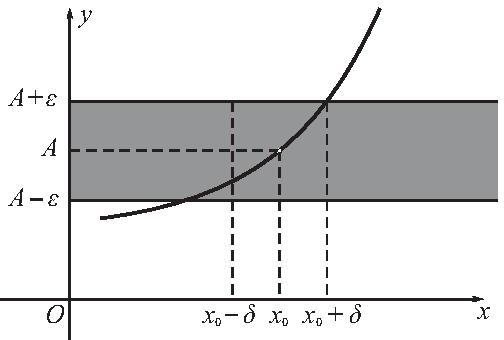
\includegraphics[scale=0.8]{pic/C-1/极限1.pdf}
	\end{center}
	\vspace*{-1em} \vspace*{-1em} 
	\caption{极限的定义图解}
\end{figure}
\vspace*{-1em}

\subsection{自变量趋于无穷大时函数的极限}
\vspace*{-1em}

\defination[函数极限2]
设函数$f(x)$在当$|x|$大于某一正数时恒有定义.如果存在常数$A$,对于任意给定的正数$\varepsilon$(不论它多么小),总存在正数$X$使得当$x$满足不等式$|x|>X$时,对应的函数值$f(x)$都满足不等式
\begin{equation}
	|f(x)-A|<\varepsilon
\end{equation}
那么常数$A$就叫做函数$f(x)$当$x \to x_0$的\dy[极限]{JX},记作
\begin{equation}
	\lim\limits_{x\to \infty}f(x)=A \quad \mbox{或} \quad f(x)\to A(x \to \infty )
\end{equation}

\subsection{无穷小与无穷大}
\vspace*{-1em}

\defination[无穷小]
如果函数$f(x)$当$x\to x_0\left(\mbox{或}x \to \infty  \right) $时的极限为$0$,那么称函数$f(x)$为当$x\to x_0\left(\mbox{或}x \to \infty  \right) $时的\dy[无穷小]{WQX}.记为
\begin{equation}
	\lim\limits_{x \to x_0}f(x)=0,\lim\limits_{x\to \infty}f(x)=0.
\end{equation}
特别地,以$0$为极限的数列${x_n}$称为$n\to \infty$时的\dy[无穷小]{WQX}.
\vspace*{1em}

\defination[无穷大]
设函数$f(x)$在$x_0$的某一去心邻域内有定义(或$|x|$趋于某一正数时有定义).如果对于任意给定的正数$M$(不论它多么大),总存在正数$\delta$(或正数$X$),只要$x$适合不等式$0<|x-x_0|<\delta$(或$|x|>X$),对应函数值$f(x)$总满足不等式
\begin{equation*}
	|f(x)|>M
\end{equation*}
那么称函数$f(x)$为当$x\to x_0\left(\mbox{或}x \to \infty  \right) $时的\dy[无穷大]{WQD}.记为
\begin{equation}
	\lim\limits_{x \to x_0}f(x)=\infty,\lim\limits_{x\to \infty}f(x)=\infty.
\end{equation}

\subsection{单侧极限}
\vspace*{-1em}

\defination[左极限]
在 $\lim\limits_{x \to x_0}f(x)=A$的定义中,把$0<|x-x_0 |<\delta$改为$x_0-\delta <x<x_0$ ,那么$A$就叫做函数$f(x)$当$x \to x_0$时的\dy[左极限]{ZJX}.记作
\begin{equation}
	\lim\limits_{x \to x_0^-}f(x)=A \quad \mbox{或} \quad f(x_0^-)=A \quad \mbox{或} \quad \lim\limits_{x \to x_0 - 0}f(x)=A
\end{equation}

\defination[右极限]
在 $\lim\limits_{x \to x_0}f(x)=A$的定义中,把$0<|x-x_0 |<\delta$改为$x_0 <x<x_0+\delta$ ,那么$A$就叫做函数$f(x)$当$x \to x_0$时的\dy[右极限]{YJX}.记作
\begin{equation}
	\lim\limits_{x \to x_0^+}f(x)=A \quad \mbox{或} \quad f(x_0^+)=A \quad \mbox{或} \quad \lim\limits_{x \to x_0 + 0}f(x)=A
\end{equation}

\subsection{利用定义求函数的极限的解题方法}
\vspace*{-1em}

\example[可以直接求得$\delta$与$\varepsilon$的关系]
任意一个$\varepsilon$满足$|f(x)-A|<\varepsilon$,都能找到一个正数$\delta$使$0 < |x - x_0| < \delta$或$|x| > \delta$ ,这就说明了$\varepsilon$与$\delta $有个对应关系,即
\begin{equation}
	\delta=\varphi(\varepsilon)
\end{equation}
\par $\delta=\varphi(\varepsilon)$这个关于$\varepsilon$的函数可以是任意的.所以我们利用极限的定义来证明某个函数的极限时,只需找到$\varepsilon$和$\delta$之间的对应关系.这时,我们可以先利用$|f(x)-A|<\varepsilon$这个条件,然后构造出 $|x - x_0| < \varphi(\varepsilon)$的形式即可.(对于求数列的极限时$\delta$换成$N$即可.)

\examples 证明下列极限\\[0.5em]
\hspace*{0.8em} $1.\,\,\lim\limits_{x \to 3}2x-1=5$

\proof  设$\exists \delta,\forall \varepsilon$,当$0<|x-3|<\delta $时,$|2x-1-5|=|2x-6|=2|x-3|<\varepsilon$\quad \quad 【构造$|x-x_0 | < \varphi (\varepsilon)$】\\[0.5em]
即$\displaystyle |x-3|<\frac{\varepsilon}{2}$,故取$\displaystyle \delta = \frac{\varepsilon}{2}$时成立,证毕.\\[1.5em]
\hspace*{0.8em} $2.\,\,\displaystyle \lim\limits_{x \to \infty }\frac{1}{x}=0$\\[1em]
\proof  设$\exists N,\forall \varepsilon$,当$|x|>N$时,$\displaystyle \left| \frac{1}{x}-0\right| =\left| \frac{1}{x}\right|<\varepsilon$\hspace{13em}【构造$|x-x_0 | < \varphi (\varepsilon)$】\\[0.5em]
即$\displaystyle |x|>\frac{1}{\varepsilon}$,故取$\displaystyle N = \frac{1}{\varepsilon}$时成立,证毕.\\

\example[不能直接求得$\delta$与$\varepsilon$的关系]
\noindent 【方法一】放缩法\vspace{0.3em}
\par 这个时候我们可以将$|f (x) - A|$进行适当的放大,使得$\delta $与$\varepsilon$的关系容易求得,一般的放缩方法有:\\[0.5em]
\noindent (1) 将分母恒大于零的部分(可以含$x$)删去;\\[0.5em]
\noindent (2) 将分子恒小于零的部分删去(可以含$x$);\\[0.5em]
\noindent (3) 将幂函数的底数部分进行放缩.

\examples 证明$\displaystyle \lim\limits_{x \to 1}\sqrt{3x+1}=2.$

\proof 设$\exists \delta,\forall \varepsilon$,当$0<|x-1|<\delta $时,$\displaystyle |\sqrt{3x+1}-2|=\frac{3(x-1)}{\sqrt{3x+1}+2}\le \frac{3}{2}|x-1|<\varepsilon$\hspace{4em}【放缩构造】\\[0.5em]
即$\displaystyle |x-1|<\frac{2}{3}\varepsilon$,又$\displaystyle \sqrt{3x+1}$定义域为$\displaystyle x>-\frac{1}{3}$,那么$\displaystyle x-1>-\frac{4}{3}$,在一定范围内有$\displaystyle |x-1|<\frac{4}{3}$\hspace{1em}【判断定义域】\\[0.5em]
故取$\displaystyle \delta = \min \left\lbrace  \frac{2}{3}\varepsilon,\frac{4}{3} \right\rbrace $时成立,证毕.\hspace{27em}【取最小值】\\

\noindent 【方法二】先设后求再取值法\vspace{0.8em}
\par 放缩不是唯一的方法,我们还可以先设后求再取$\delta $最小值.\\[0.3em]
\noindent (1) 先化简式子,且含$|x-a|$项,这个时候可以用该方法;\\[0.5em]
\noindent (2) 设$\delta $的值为$f(a)$ (可以含$a,x$,也可以是常数);\\[0.5em]
\noindent (3) 解出$x$的范围,对非$|x - a|$的项进行放缩,将式子放大,同时使得非$|x - a|$的项转换为常量;\\[0.5em]
\noindent (4) 反解出$\delta = \varphi (\varepsilon)$;\\[0.5em]
\noindent (5) 取$\delta = \min \lbrace f(a),\varphi(\varepsilon)\rbrace$.\vspace{0.5em}
\par 当然通常放缩法和先设后求再取值法会结合用,这样就可以解决大部分题目.
\par 但是在后面的证明过程中,一般简单的函数极限可以直接用,所以一般情况下不会用定义证明极限.

\examples 证明$\lim\limits_{x \to a}x^2=a^2$

\proof 由于$|x^2-a^2|=|(x-a)(x+a)|=|x-a|\cdot |x+a| $,\hspace{16em}【找到$|x-a|$项】\\[0.5em]
设$\displaystyle |x-a|<\frac{1}{2}$,则$\displaystyle |x+a|=|x-a+2a|\le |x-a|+|2a|<\frac{1}{2}+|2a|.$ \hspace*{2em}【赋值$|x-a|$项,并放缩得出未知项的范围】\\[0.5em]
所以,设$\exists \delta,\forall \varepsilon$,当$0<|x-1|<\delta $时,$\displaystyle |x^2-a^2|=|x-a|\cdot |x+a|<\left( \frac{1}{2}+|2a|\right)|x-a|<\varepsilon $,\\[0.5em]
即$\displaystyle|x-a|<\frac{\varepsilon}{\frac{1}{2}+2|a|}$.\hspace{29em}【反解出$|x-a|$的范围】\\[0.5em]
故取$\displaystyle \delta = \min \left\lbrace  \frac{\varepsilon}{\frac{1}{2}+2|a|},\frac{1}{2} \right\rbrace $时成立,证毕.\hspace{26em}【取最小值】

\subsection{证明函数的极限不存在的方法}
\vspace*{-1em}

\theorem[序列极限]
设函数$f (x)$在$a$点的一个空心邻域内有定义,并且$\lim\limits_{x \to a}f(x)=l$.假若是一串在该空心邻域内取值的序列,且
\begin{equation*}
	\lim\limits_{n \to \infty}x_n=a
\end{equation*}
则有
\begin{equation}
	\lim\limits_{n \to \infty}f(x_n)=l
\end{equation}
\par 这个定理为我们提供了一种\textbf{证明函数极限不存在的办法}:对于一个定义在$a$点的某空心邻域内的函数$f(x)$,如果能找到两串序列$\lbrace x'_n \rbrace $与$\lbrace x''_n\rbrace$它们都在$a$的该空心邻域内取值,且当$n\to \infty $时都以$a$为极限,而极限$\lim\limits_{n \to \infty }x'_n$与 $\lim\limits_{n \to \infty }x''_n$都存在但不相等,则$f(x)$在$x \to a$时不可能有极限.\vspace*{1em}

\example[证明函数的极限不存在]
\vspace*{-1em} \examples 证明:函数$\displaystyle \sin \frac{1}{x}$在$x\to 0$时没有极限.

\proof 取$\displaystyle x'_n=\frac{1}{2n\pi }$,则$\displaystyle \sin \frac{1}{x'_n}=0$;而取$\displaystyle x''_n=\frac{1}{2n\pi+\frac{\pi}{2} }$,则$\displaystyle \sin \frac{1}{x'_n}=1.$\\[0.5em]
这时由于$n \to \infty \Rightarrow x'_n\to 0,x''_n \to 0, $且
\begin{equation*}
	\lim\limits_{n \to \infty} \sin \frac{1}{x'_n} \ne \lim\limits_{n \to \infty} \sin \frac{1}{x''_n} 
\end{equation*}
因此,函数$\displaystyle \sin \frac{1}{x}$在$x\to 0$时没有极限.

\section{利用极限运算法则和两个准则求极限}
\subsection{极限运算法则}
\vspace*{-1em}

\theorem[极限运算法则1]
两个无穷小的和是无穷小.

\tl 有限个无穷小的和是无穷小.
\newpage
\theorem[极限运算法则2]
有界函数与无穷小的乘积是无穷小.

\tl 常数与无穷小的乘积是无穷小.

\tl 有限个无穷小的乘积是无穷小.\vspace*{1em}

\theorem[极限运算法则3]
如果$\lim f(x) = A, \lim g(x) = B$(这些函数都必须存在极限),那么
\begin{equation}
	\lim [f(x)\pm g(x)]=\lim f(x)\pm \lim g(x)=A \pm B
\end{equation}
\begin{equation}
	\lim[f(x)\cdot g(x)]=\lim f(x)\cdot \lim g(x)=A\cdot B
\end{equation}
若$B\ne 0$,那么
\begin{equation}
	\lim \left[ \frac{f(x)}{g(x)}\right] =\frac{\lim f(x)}{\lim g(x)}=\frac{A}{B}
\end{equation}

\tl 如果$\lim f(x)$存在,而$c$为常数,那么
\begin{equation}
	\lim [cf(x)]=c \lim f(x)
\end{equation}

\tl 如果$\lim f(x)$存在而$n$为正整数,那么
\begin{equation}
	\lim [f(x)]^n=[\lim f(x)]^n
\end{equation}

\theorem[极限运算法则4]
如果$\varphi(x) \ge \psi(x),$而$\lim \varphi(x)=A,\lim \psi(x)=B,$则$A \ge B.$\vspace*{1em}

\subsection{极限运算准则}
\vspace*{-1em}

\theorem[单调有界数列极限一定存在]
(1)  \quad 若$x_{n+1} \le x_n(n\mbox{为正整数})$,且$x_n \ge m,$则$\lim\limits_{n \to \infty }x_n = A $存在,且$A \ge m$;
\par (2)  \quad 若$x_{n+1} \ge x_n(n\mbox{为正整数})$,且$x_n \le M,$则$\lim\limits_{n \to \infty }x_n = A $存在,且$A \le M$.

\theorem[夹逼定理]
设$g(x) \le f(x) \le h(x)$,若$\lim\limits_{x \to m}g(x)=A,\lim\limits_{x \to m}=A,(-\infty \le m \le +\infty)$则$\lim\limits_{x \to m}f(x)=A.$\vspace*{1em}

\subsection{例题}
\vspace*{-1em}

\example[利用极限运算法则和两个准则求极限]\vspace*{-1em}
\examples 证明:$\lim\limits_{n \to \infty}q^n=0.(|q|<1)$

\proof 设$\displaystyle |q|=\frac{1}{1+a},a>0,$则$\displaystyle 0< q^n=\frac{1}{(1+a)^n}=\frac{1}{C^0_na^0=C^1_na^1+C^2_na^2+\cdots+C^n_na^n}<\frac{1}{C^1_na^1}=\frac{1}{na}.$\\[0.5em]
又$\displaystyle \lim\limits_{n \to \infty}\frac{1}{na}=0,\lim\limits_{n\to \infty}0=0,$由夹逼定理可得
\begin{equation*}
	\lim\limits_{n\to \infty}0 \le \lim\limits_{n \to \infty}q^n \le \lim\limits_{n \to \infty}\frac{1}{na}
\end{equation*}
故$\lim\limits_{n \to \infty}q^n=0.$\vspace*{1em}

\examples 证明:$\displaystyle a_n=\frac{a^n}{n!}(a\mbox{是大于1的任意常数})$存在极限.

\proof 当$n>[a]+1$时,有
\begin{equation*}
	0\le a_n =\frac{a^{[a]}}{[a]!}\cdot \frac{a}{[a]+1}\cdot \frac{a}{[a]+2}\cdot \,\,\cdots \,\,\cdot \frac{a}{n}<\frac{a^{[a]}}{[a]!}\cdot \frac{a}{n}
\end{equation*}
注意到$\displaystyle \frac{a^{[a]}}{[a]!}$是一个常数,所以$\displaystyle \lim\limits_{n \to \infty}\frac{a^{[a]}}{[a]!}\cdot \frac{a}{n}=0,$由夹逼定理可得
\begin{equation*}
	\lim\limits_{n \to \infty}a_n=0.
\end{equation*}

\examples 设常数$a>1,$对于任意自然数$k$,证明:
\begin{equation*}
	\lim\limits_{n \to \infty}\frac{n^k}{a^n}=0.
\end{equation*}
\hspace*{-0.5em}\proof 令$t=a-1$,则$t>0$,那么
\[
a_n=(1+t)^n=1+nt+\frac{n(n-1)}{2!}t^2+\cdots+\frac{n(n-1)\cdot(n-k)}{(k+1)!}t^{k+1}+\cdots+t^n,
\]
因此,当$n>1$时,$\displaystyle a^n>\frac{n(n-1)\cdots(n-k)}{(k+1)!}t^{k+1}$,于是
\[
0 \le \frac{n^k}{a^n}\le \frac{n^k}{\displaystyle \frac{n(n-1)\cdots(n-k)}{(k+1)!}t^{k+1}}=\frac{(k+1)!}{t^{k+1}}\cdot \frac{n^k}{n(n-1)\cdots(n-k)}=\frac{(k+1)!}{t^{k+1}}\cdot\frac{n^k}{\lambda_{k+1}n^{k+1}+\lambda_kn^k+\cdots+\lambda_1n+\lambda_0}
\]
其中$\lambda_0,\lambda_1,\cdots,\lambda_{k+1}$均为非零常数.注意到$\displaystyle \frac{(k+1)!}{t^{k+1}}$为常数,则
\begin{equation*}
	\begin{split}
		&\quad \, \lim\limits_{n \to \infty}\frac{(k+1)!}{t^{k+1}}\cdot\frac{n^k}{\lambda_{k+1}n^{k+1}+\lambda_kn^k+\cdots+\lambda_1n+\lambda_0}\\
		&=\lim\limits_{n \to \infty}\frac{(k+1)!}{t^{k+1}}\cdot\frac{1}{n}\cdot \frac{n^k}{\lambda_{k+1}+\lambda_kn^{-1}+\cdots+\lambda_1n^{-k}+\lambda_0n^{-k-1}}=0
	\end{split}
\end{equation*}
因此,由夹逼定理可得
\begin{equation*}
	\lim\limits_{n \to \infty}\frac{n^k}{a^n}=0.
\end{equation*}

\section{利用等价无穷小求极限}
\subsection{无穷小的分类}
\vspace*{-1em}

\defination[无穷小的分类]
设$\alpha,\beta $是同一变化过程中的无穷小,$\displaystyle \lim \frac{\beta}{\alpha}$是这一过程的极限,$c$为常数,那么\\[0.5em]
\noindent (1) \quad $\displaystyle \lim \frac{\beta }{\alpha}=0$,则称$\beta $是$\alpha $的\dy[高阶无穷小]{GJWQX},记作$\beta = o(\alpha)$.\\[0.5em]
\noindent (2) \quad  $\displaystyle \lim \frac{\beta }{\alpha}=\infty$,则称$\beta $是$\alpha $的\dy[低阶无穷小]{DJWQX1}.\\[0.5em]
\noindent (3) \quad  $\displaystyle \lim \frac{\beta }{\alpha}=c \ne 0$,则称$\beta $是$\alpha $的\dy[同阶无穷小]{TJWQX}.\\[0.5em]
\noindent (4) \quad  $\displaystyle \lim \frac{\beta }{\alpha}=1$,则称$\beta $是$\alpha $的\dy[等价无穷小]{DJWQX2},记作$\beta \sim \alpha$.\\[0.5em]
\noindent (3) \quad  $\displaystyle \lim \frac{\beta }{\alpha^k}=c \ne 0$,则称$\beta $是$\alpha $的\dy[$k$阶无穷小]{KJWQX}.

\warn[
{\large \bf 0与``0"的区别}\vspace*{0.5em}\\
\hspace*{1em}(1)\quad ``0"指的是无穷小,设$\alpha$是某一变化过程中的无穷小,也就是说$x$趋于某一值时,极限为0.\vspace*{0.5em}\\
\hspace*{1em}(2)\quad 当0指的是实数0时,$\lim 0 \cdot f(x)=0$,这与$f(x)$无关,即使$\lim f(x)=\infty$,其结果仍然是0,因为0在这里是实数,而不是无穷小.
]


\subsection{常见的等价无穷小}
\vspace*{-1em}

\theorem[常见的等价无穷小]
以下等价无穷小均为$x \to 0$这一变化过程,其中$x$也可替换为一个函数,即$f(x) \to 0$的情况也适用.
\begin{equation}
	\tan x \sim \sin x \sim x \sim \arcsin x \sim \arctan x
\end{equation}
\begin{equation}
	\ln (1+x) \sim x
\end{equation}
\begin{equation}
	x \sim \e^x -1
\end{equation}
\begin{equation}
	1-\cos x \sim \frac{x^2}{2}
\end{equation}
\begin{equation}
	\sec x -1 =\frac{1}{\cos x}-1 \sim \frac{x^2}{2}
\end{equation}
\begin{equation}
	(1+x)^a-1 \sim ax
\end{equation}
\begin{equation}
	a^x-1 \sim \ln a \cdot x \,(a>0,a \ne 1)
\end{equation}
\subsection{等价无穷小求极限的本质}
等价无穷小求极限本质上是极限与1的相乘,而有等价无穷小的定义,1可以换成极限$\displaystyle 1=\lim\limits_{x \to x_0}\frac{\alpha }{\beta}$,再运用极限乘法运算法则计算即可.

\example[等价无穷小的误用]\vspace*{-1em}
\examples \label{例 1.8}求极限$\displaystyle \lim\limits_{x \to 0}\frac{\tan x -\sin x}{\sin^3 x}$.

\errsolve  由于$\tan \sim \sin x \sim x$得$\displaystyle \lim\limits_{x \to 0}\frac{\tan x -\sin x}{\sin^3 x}=\lim\limits_{x \to 0}\frac{x-x}{\sin^3 x}=\lim\limits_{x \to 0}0=0.$

\errreason  在运用等价无穷小的时候没有考虑极限运算法则成立的条件.

\solvereason $\displaystyle \lim\limits_{x \to 0}\frac{\tan x -\sin x}{\sin^3 x}=\lim\limits_{x \to 0}\frac{\tan x}{\sin^3 x} - \lim\limits_{x \to 0}\frac{\sin x}{\sin^3 x}$实际上运用了法则$\lim [f(x)-g(x)]=\lim f(x)-\lim g(x),$\\[1em]即完整的错解解题步骤应为
\begin{equation*}
	\lim\limits_{x \to 0}\frac{\tan x -\sin x}{\sin^3 x}=\lim\limits_{x \to 0}\frac{\tan x}{\sin^3 x} - \lim\limits_{x \to 0}\frac{\sin x}{\sin^3 x}
	=\lim\limits_{x \to 0}\frac{\tan x}{\sin^3 x}\cdot \lim\limits_{x \to 0} \frac{x}{\tan x}-\lim\limits_{x \to 0}\frac{x}{\sin^3 x}
\end{equation*}
而极限运算法则成立的条件是$\lim f(x),\lim g(x)$存在,而$\displaystyle \lim\limits_{x \to 0}\frac{\tan x}{\sin^3 x}$不存在,因此解题错误.

\solve $\displaystyle \lim\limits_{x \to 0}\frac{\tan x -\sin x}{\sin^3 x}=\lim\limits_{x \to 0}\frac{\sin x(\sec x-1)}{\sin^3 x}=\lim\limits_{x \to 0}\frac{\sec x-1}{\sin^2 x} \cdot \lim\limits_{x \to 0}\frac{\frac{x^2}{2}}{\sec x -1} \cdot \lim\limits_{x \to 0}\frac{\sin x^2}{x^2}
=\frac{\frac{x^2}{2}}{x^2}=\frac{1}{2}.$\vspace*{1em}

\examples 求极限$\displaystyle \lim_{x \to 0} \frac{\sin \left(x^2 \sin{\frac{1}{x}}\right) }{x}.$

\errsolve $\displaystyle \lim_{x \to 0}\frac{\sin \left(x^2 \sin{\frac{1}{x}}\right) }{x}=\lim_{x \to 0}\frac{x^2 \sin \frac{1}{x}}{x}=\lim_{x \to 0}x\sin\frac{1}{x}=0.$

\errreason 对极限概念的理解不清晰,不仔细,没有严格判断等价无穷小的定义式是否满足极限的定义.

\solvereason 实际上,该错误解答的完整版本应该为:
\[
\lim_{x \to 0} \frac{\sin \left(x^2 \sin{\frac{1}{x}}\right) }{x}=\lim_{x \to 0} \frac{\sin \left(x^2 \sin{\frac{1}{x}}\right) }{x}\cdot\frac{x^2\sin \frac{1}{x}}{\sin \left( x^2 \sin \frac{1}{x}\right) }=\lim_{x \to 0}\frac{x^2\sin\frac{1}{x}}{x}=\lim_{x \to 0}x\sin \frac{1}{x}=0.
\]
但是极限
\[
\lim_{x \to 0}\frac{x^2\sin \frac{1}{x}}{\sin \left( x^2\sin \frac{1}{x}\right) }
\]
中,若$\displaystyle \sin \frac{1}{x}$取0,则这个极限式无意义(分母为0).故$\displaystyle x \ne \frac{1}{k \pi}(k \in Z).$\hspace*{12.5em}【判断定义域】\\[0.5em]
\hspace*{2em}这样的话,在点$x = 0$的任何一个去心邻域中都有无穷多个点没有定义,所以不存在一个去心邻域满足该极限式,
故极限不存在.\hspace*{24em}【判断是否能找到满足的去心邻域】\\[0.5em]
这里再次强调一下0与``0"的区别: 分母为0的时候并不是指无穷小量,而是真正意义上的0.

\solve 设$\exists \delta, \forall \varepsilon,$使得当$|x-0|<\delta$时,$\displaystyle \left| \frac{\sin \left( x^2\sin\frac{1}{x}\right) }{x}-0\right|<\varepsilon$,\\[0.5em]
由不等式$|\sin x|\le |x|$,得
\[
\left| \frac{\sin \left( x^2\sin\frac{1}{x}\right) }{x}\right| \le \left| \frac{ \left( x^2\sin\frac{1}{x}\right) }{x}\right| =\left| x \sin \frac{1}{x} \right|.
\]
由$\displaystyle \left| \sin \frac{1}{x} \right| \le 1$,得
\[
\left| \frac{\sin \left( x^2\sin\frac{1}{x}\right) }{x}\right| \le \left| \frac{ \left( x^2\sin\frac{1}{x}\right) }{x}\right| =\left| x \sin \frac{1}{x} \right|.\le |x|<\varepsilon
\]

\subsection{例题}
\vspace*{-1em}
\example[等价无穷小的运用]
在下面的例题中,为了方便,省略了含有等价无穷小本质的式子.但是建议读者在实际做题的过程中还是要写完整,方便利用定义检查式子的合理性.

\examples 求极限$\displaystyle \lim_{x \to \infty}\left(\cos \frac{3}{x} \right)^{x^2} $

\solve 令$\displaystyle t=\frac{1}{x}$,则$x=\dfrac{1}{t},x\to \infty ,t \to 0.$

\newpage 
\vspace*{-2em}
\[
\lim_{x \to \infty}\left(\cos \frac{3}{x} \right)^{x^2} =\lim_{t \to 0}(\cos 3t)^{\frac{1}{t^2}}=\lim_{t \to 0}\left[\left( 1-2\sin^2\frac{3t}{2}\right)^{\frac{1}{2\sin^2\frac{3t}{2}}} \right]^{\frac{2\sin^2\frac{3t}{2}}{t^2}} =\e^{\displaystyle -\lim_{t \to 0}\frac{2\sin^2\frac{3t}{2}}{t^2}}
\]
因为$\displaystyle \lim_{t \to 0}\frac{2\left( \displaystyle \frac{3t}{2}\right)^2 }{t^2}=\frac{9}{2},\,\therefore \lim_{x \to \infty }\left(\cos \frac{3}{x} \right)^{x^2}=\e^{ \displaystyle  -\lim_{t \to 0}\frac{2\sin^2\frac{3t}{2}}{t^2}}=\e ^{-\frac{9}{2}} $

\solveother 令$\displaystyle t=\frac{1}{x}$,则$\displaystyle x=\frac{1}{t},x\to \infty ,t \to 0.$
\[
\lim_{x \to \infty}\left( \cos \frac{3}{x}\right)^{x^2} =\lim_{t \to 0}(\cos 3t)^{\frac{1}{t^2}}=\e^{\lim\limits_{t \to 0}\ln(\cos 3t)^{\frac{1}{t^2}}}
\]
\[
\because \lim\limits_{t \to 0}\frac{1}{t^2}\ln(\cos 3t)=\lim\limits_{t \to 0}\frac{1}{t^2}\ln (\cos 3t)=\lim\limits_{t \to 0}\frac{1}{t^2}\ln \left[1+\left(-2\sin^2\frac{3t}{2}\right)\right]=\lim_{t \to 0}\frac{-2\sin^2\frac{3t}{2}}{t^2}=\lim\limits_{t \to 0}\frac{-2\left(\frac{3t}{2}\right)^2}{t^2}=-\frac{9}{2}.
\]
\[
\therefore \lim_{x \to \infty}\left( \cos \frac{3}{x}\right)^{x^2}=\lim\limits_{t \to 0}(\cos 3t)^{\frac{1}{t^2}}=\e^{\lim\limits_{t \to 0}\ln(\cos 3t)^{\frac{1}{t^2}}}=\e^{-\frac{9}{2}}.
\]

\inference[等价无穷小类型\uppercase\expandafter{\romannumeral1}]
以上是利用两种等价无穷小的解法,下面对这两种等价无穷小的用法归类.(这两个极限选一个用即可).若一个极限表达式有下列的形式(或者经过换元、取对数等方法变成这种形式),则很有可能用到这两种极限.
\begin{equation}
	\lim f(x)^{g(x)}
\end{equation}
其中$\lim f(x)=1,\lim g(x)$存在.

解法一\qquad 变形为:
\begin{equation}
	\lim\big[1+\big(f(x)-1\big)\big]^{g(x)}=\lim\big[1+\big(f(x)-1\big)\big]^{\frac{g(x)[f(x)-1]}{f(x)-1}}=\e^{\lim g(x)\cdot [f(x)-1]}
\end{equation}
而此时$\lim g(x) \cdot [f(x)-1]$是容易求得的.


解法二\qquad 变形为:
\begin{equation}
	\lim\big[1+\big(f(x)-1\big)\big]^{g(x)}=\e^{\lim \ln[1+\left( f(x)-1\right) ]}=\e^{\lim g(x)\cdot [f(x)-1]}
\end{equation}
而此时$\lim g(x) \cdot [f(x)-1]$也是容易求得的.

\examples 已知函数$f(x)$满足$\displaystyle \lim_{x \to 0}\frac{\sqrt{1+f(x)\sin 2x}-1}{\e^{3x}-1}=2$,求$\displaystyle \lim_{x \to 0}f(x).$

\solve $\displaystyle \lim_{x \to 0}\frac{\sqrt{1+f(x)\sin 2x}-1}{\e^{3x}-1}=\lim\limits_{x \to 0}\frac{1/2f(x)\sin 2x}{3x}=\lim_{x \to 0}\frac{1/2f(x)2x}{3x}=\frac{1}{3}\lim_{x\to 0}f(x)=2.$
\[
\therefore \lim_{x \to 0}f(x)=6.
\]

下面给出一个较难看出错误的例题.

\examples \label{例 1.12}求极限$\displaystyle \lim_{x \to 0}\left[ \frac{(1+x)^{\frac{1}{x}}}{\e}\right]^{\frac{1}{x}}.$

\errsolve $\displaystyle \lim_{x \to 0}\left[ \frac{(1+x)^{\frac{1}{x}}}{\e}\right]^{\frac{1}{x}}=\lim_{x \to 0}\left[ \frac{\e}{\e}\right]^{\frac{1}{x}}=1.$

\errreason 在运用等价无穷小的时候没有考虑极限运算法则成立的条件.

\solvereason $\displaystyle \lim_{x \to 0}\left[ \frac{(1+x)^{\frac{1}{x}}}{\e}\right]^{\frac{1}{x}}=\e^{\lim\limits_{x \to 0}\frac{1}{x}\ln\frac{(1+x)^{\frac{1}{x}}}{\e}},$
\[
\lim_{x \to 0}\frac{1}{x}\ln\frac{(1+x)^{\frac{1}{x}}}{\e}=\lim\limits_{x \to 0}\frac{1}{x}\left[ \ln(1+x)^{\frac{1}{x}} -\ln \e\right]=\lim\limits_{x \to 0}\frac{1}{x}\cdot\lim\limits_{x \to 0}\left[ \ln(1+x)^{\frac{1}{x}} -\ln \e\right]=\lim_{x \to 0}\frac{1}{x} \cdot \lim\limits_{x \to 0} \left[ \ln \e -\ln \e \right]=0.
\]
实际上,在$\displaystyle \lim\limits_{x \to 0}\frac{1}{x}\left[ \ln(1+x)^{\frac{1}{x}}-\ln \e \right]=\lim\limits_{x \to 0}\frac{1}{x}\cdot\lim\limits_{x \to 0}\left[ \ln(1+x)^{\frac{1}{x}} -\ln \e\right]$中用到了$\lim \big[f(x)\cdot g(x)\big]=\lim f(x) \cdot \lim  g(x)$,即用到了极限运算法则,而$\displaystyle \lim_{x \to 0}\frac{1}{x}$不存在,因此这种运算错误.

\solve $\displaystyle \lim_{x \to 0}\left[ \frac{(1+x)^{\frac{1}{x}}}{\e}\right]^{\frac{1}{x}}=\lim_{x \to 0}\left\lbrace1+\left[\frac{(1+x)^{\frac{1}{x}}}{\e}-1\right]\right\rbrace^{\frac 1x}=\lim_{x \to 0}\left\lbrace1+\left[\frac{(1+x)^{\frac{1}{x}}}{\e}-1\right]\right\rbrace^{ \frac{1}{(1+x)^{\frac 1x}-1}\cdot \frac{(1+x)^{\frac 1x}-1}{x}},$
\[
\because \lim\limits_{x \to 0}\left[\frac{(1+x)^{\frac{1}{x}}}{\e}-1\right]=0,\therefore \lim_{x \to 0}\left\lbrace1+\left[\frac{(1+x)^{\frac{1}{x}}}{\e}-1\right]\right\rbrace^{ \frac{1}{(1+x)^{\frac 1x}-1}\cdot \frac{(1+x)^{\frac 1x}-1}{x}}=\e^{\lim\limits_{x\to 0}\frac{(1+x)^\frac 1x-1}{x}},
\]
\[
\because \lim\limits_{x\to 0}\frac{\frac{(1+x)^\frac 1x}{\e}-1}{x}=\lim\limits_{x\to 0}\frac{(1+x)^\frac 1x-\e}{\e x}=\lim\limits_{x \to 0}\frac{\e^{\frac{1}{x}\ln(1+x)}-\e}{\e x}\xlongequal[]{\e^x-1 \sim x} \lim\limits_{x \to 0}\frac{\frac{1}{x}\ln(1+x)-1}{x}=\lim_{x \to 0}\frac{\ln (1+x)-x}{x^2}
\]
\[
\xlongequal[]{\ln(1+x)-x\sim-\frac{1}{2}x^2} \lim\limits_{x \to 0}\frac{-\frac{1}{2}x^2}{x^2}=-\frac{1}{2}
\]
\[
\therefore \lim_{x \to 0}\left[ \frac{(1+x)^{\frac{1}{x}}}{\e}\right]^{\frac{1}{x}}=\e^{\lim\limits_{x\to 0}\frac{(1+x)^\frac 1x-1}{x}}=\e^{-\frac{1}{2}}=\frac{\sqrt{\e}}{\e}.
\]

\inference[等价无穷小求极限]\vspace*{-1em}
\begin{enumerate}
	\item 判断并构造等价无穷小的类型(7 种);
	\item 利用等价无穷小求极限的本质列出计算式;
	\item 判断等价无穷小的极限式中能否找到满足定义域的去心邻域使得极限存在:
	\begin{enumerate}[(i)]
		\item 若存在,则利用等价无穷小解题;
		\item 若不存在,则用其它方法求解(如利用函数定义、夹逼准则等).
	\end{enumerate}
	\item 检验计算的每一步是否都符合极限运算法则的前提条件.
\end{enumerate}
\vspace*{-2em}
\warn[
\hspace*{2em}1. 以上等价无穷小都只在$x\to 0$的情况下才成立,$x$趋于其它值时不成立.\\
\hspace*{2em}2. 只有等价无穷小的定义式存在极限的前提下,即在函数$f (x)$的定义域内能找到一个完整的去心邻域,$x$才可以用任意函数$f(x)$替换.若等价无穷小的定义式都不存在极限,又谈何等价无穷小.\\
下面给出常见的一些不可以用等价无穷小替换的函数.\vspace*{1em}\\
\examples $\displaystyle x \to 0,\sin\left(x \sin \frac 1x\right) \not \sim x\sin \frac{1}{x},\sin\left(x\cos \frac 1x\right)\not \sim x \cos \frac 1x$\\
\hspace*{2em}3. 在运用等价无穷小计算极限的时候要特别要注意在替换的过程中只有符合极限的运算法则,才可以进行
替换(通常极限的运算法则不明显,需要仔细计算),前面已经给出了两个详细的例子.
]

\section{函数连续性}
\subsection{函数连续性的定义}
\vspace*{-1em}

\defination[函数在某点的连续性\uppercase\expandafter{\romannumeral1}]
设函数$y=f(x)$在点$x_0$的某一邻域内有定义,如果
\begin{equation}
	\lim\limits_{\Delta x \to 0}\Delta y=\lim\limits_{\Delta x \to 0}\big[f(x_0+\Delta x)-f(x_0)\big]=0.
\end{equation}
那么就称函数$y=f(x)$在点$x_0$处\dy[连续]{LX}.

\defination[函数在某点的连续性\uppercase\expandafter{\romannumeral2}]
设函数$y=f(x)$在点$x_0$的某一邻域内有定义,如果
\begin{equation}
	\lim\limits_{x \to x_0} f(x)=f(x_0).
\end{equation}
那么就称函数$y=f(x)$在点$x_0$处\dy[连续]{LX}.\vspace*{1em}

即$f(x)$在点$x_0$处连续$\Longleftrightarrow \forall \varepsilon>0,\exists \delta>0,$当$|x-x_0|<\delta$时,都有$|f(x)-f(x_0)|<\varepsilon$

\defination[左连续]
如果$\lim\limits_{x \to x_0^-}f(x)=f(x_0^-)$存在且等于$f(x_0)$,即$f(x_0^-)=f(x_0)$,那么就称函数$y=f(x)$在点$x_0$处\dy[左连续]{ZLX}.

\defination[右连续]
如果$\lim\limits_{x \to x_0^+}f(x)=f(x_0^+)$存在且等于$f(x_0)$,即$f(x_0^+)=f(x_0)$,那么就称函数$y=f(x)$在点$x_0$处\dy[右连续]{YLX}.

\warn[\hspace*{2em}函数在某点连续的充要条件是在该点的左极限和右极限都存在且都等于函数该点处的函数值.或者说函数在该点既左连续又右连续.(证明函数在某点处是否连续的方法)]


\defination[函数在某个区间的连续性]
在区间上每一点都连续的函数,叫做在该区间上的连续函数,或者说函数在该区间上连续.如果区间包括端点,那么函数在右端点是指右端点的左连续,在左端点是指左端点的右连续.

\textbf{连续函数的图形是一条连续而不间断的线(可能是直线,也可能是曲线).}

\subsection{函数的间断点}
\vspace*{-1em}

\defination[函数的间断点]
设函数$y=f(x)$在点$x_0$的某一邻域内有定义.在此前提条件下,如果函数有下列三种情况之一:\\[0.5em]
(1) 在$x=x_0$处没有定义;\hspace{12em}(2) 虽在$x=x_0$处有定义,但是$\displaystyle \lim\limits_{x \to x_0}f(x)$不存在;\\[0.5em]
(3) 虽在$x=x_0$处有定义,$\displaystyle \lim\limits_{x \to x_0}f(x)$存在,但$\displaystyle \lim_{x \to x_0}f(x) \ne f(x_0)$.\\[0.5em]
那么就称函数$f(x)$在点$x_0$处不连续,而点$x_0$称为函数$f(x)$的\dy[不连续点]{BLXD}或\dy[间断点]{JDD}.

如果$x_0$是函数$f(x)$的间断点,但左极限$f(x_0^-)$和右极限$f(x_0^+)$都存在,那么点$x_0$就称为函数$f(x)$的\dy[第一类间断点]{DYLJDD},不是第一类间断点的任何间断点都是\dy[第二类间断点]{DELJDD}.常见的具体分类见下表\ref{函数间断点的分类}.
\begin{table}[!htb]
	\centering
	\renewcommand{\arraystretch}{1}
	\setlength{\tabcolsep}{14mm}{
		\begin{tabular}{cc}
			\toprule[1.5pt] 
			第一类间断点 & 第二类间断点 \\
			\midrule
			可去间断点 & 无穷间断点\\
			跳跃间断点 & 震荡间断点\\
			\bottomrule[1.5pt]
		\end{tabular}  
	}
	\caption{函数间断点的分类}
	\renewcommand{\arraystretch}{1}
	\label{函数间断点的分类}
\end{table} 
\vspace*{-3em}

\defination[无穷间断点]
若$x_0$是函数$f(x)$的间断点,且$\lim\limits_{x \to x_0}f(x)=\infty $,那么我们称点$x_0$是函数的\dy[无穷间断点]{WQJDD}.\vspace*{1em}

\simpleexamples $\displaystyle x=\frac{\pi}{2}$是函数$y=\tan x$的无穷间断点.

\defination[振荡间断点]
若$x_0$是函数$f(x)$的间断点,且当$x \to x_0$时,函数值在多个值之间变动无穷多次,那么我们称点$x_0$是函数$f(x)$的\dy[振荡间断点]{ZDJDD}.\vspace*{1em}

\simpleexamples $\displaystyle x = 0$是函数$\displaystyle y =\sin\frac{1}{x}$的振荡间断点.
\warn[
\hspace*{2em} 若点$x_0$是函数$f(x)$的振荡间断点,那么在函数$f(x)$在点$x_0$处的任意的去心邻域都无确定的值.
进一步说,如果函数$f(x)$的导函数是$f'(x)$,点$x_0$是导函数$f'(x)$的振荡间断点,那么在$x_0$的任意去心邻域中函数$f(x)$的导数都不存在.
]
\vspace*{-1em}

\defination[可去间断点]
若点$x_0$是函数$f(x)$的间断点,且$f(x)$在点$x_0$处没有定义,而$\lim\limits_{x \to x_0}f(x)=f(x_0),$那么我们称点$x_0$是函数$f(x)$的\dy[可去间断点]{KQJDD}.\vspace*{1em}

\simpleexamples $\displaystyle x=1$是函数$\displaystyle y=\frac{x^2-1}{x-1}$的可去间断点.

\defination[跳跃间断点]
若点$x_0$是函数$f(x)$的间断点,且$f(x)$在点$x_0$处有定义,而$f(x_0^-)=f(x_0^+)$,那么我们称点$x_0$是函数$f(x)$的\dy[跳跃间断点]{TYJDD}.

\simpleexamples $\displaystyle x=0$是函数
$
\displaystyle
\begin{cases}
	x-1&,x<0\\
	0&,x=0\\
	x+1&,x>0
\end{cases}
$
的跳跃间断点.

\begin{tcolorbox}[sidebyside,colframe=red!75!black, colback=yellow!10!white,title=注意,sidebyside align=top seam,
	righthand width=4cm,fonttitle =\CJKfamily{heiti}]
	\hspace*{2em} 可去间断点的定义是左右极限相等即可,与函数在该点处是否有定义无关.关于这个很容易犯错,下面给出一个例子详细说明.
	\[
	f(x)=
	\begin{cases}
		x^2-1,&x<-3\\
		-1,&x=-3\\
		-3x-1,&-3<x\le 0
	\end{cases}
	\]
	如图,$\lim\limits_{x \to -3^-}f(x)=\lim\limits_{x \to -3^-}x^2-1=(-3)^2-1=8.$\\[0.5em]
	$\lim\limits_{x \to -3^+}=\lim\limits_{x \to -3^+}-3x-1=(-3)^2-1=8.$\\[0.5em]
	所以,$\lim\limits_{x \to -3^-}f(x)=\lim\limits_{x \to -3^+}f(x)=8 \neq f(-3).$\\[0.5em]
	即$x=-3$是函数$f(x)$的可去间断点.
	\tcblower
	\centering
	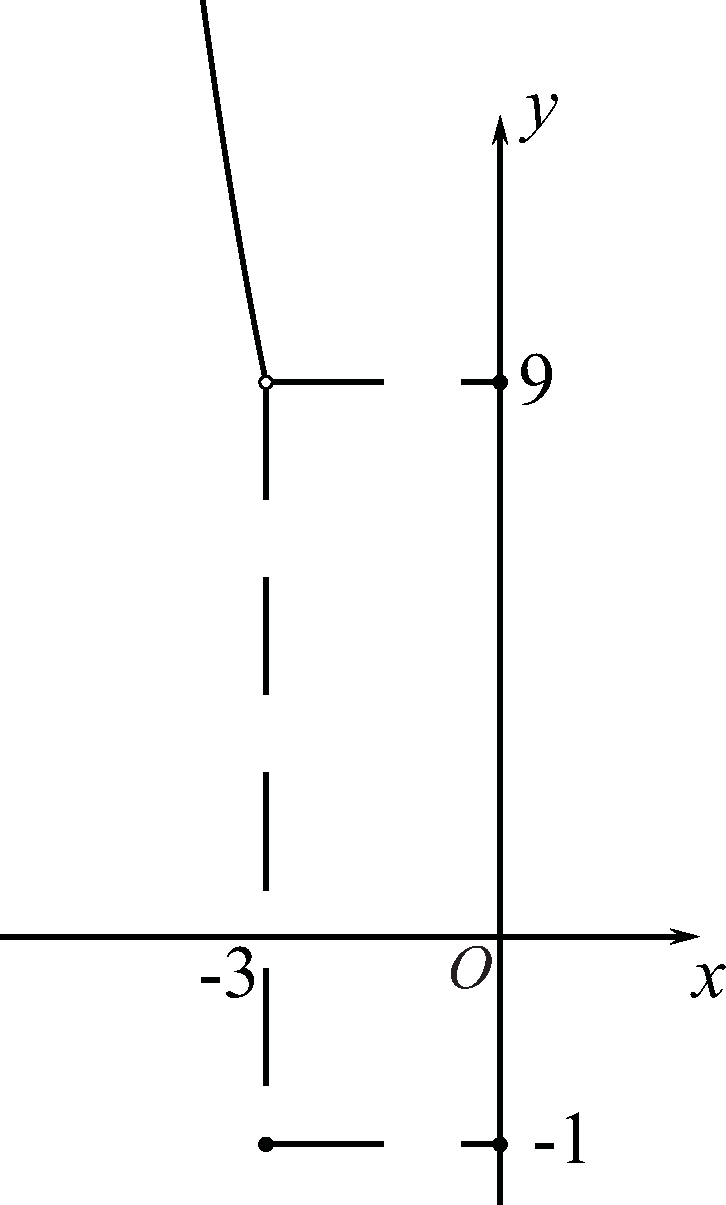
\includegraphics[width=\linewidth]{pic/C-1/可去间断点.pdf}
\end{tcolorbox}

\inference[判断间断点的类型]
\begin{center}
	\begin{tikzpicture}[node distance=1.2cm]
		%定义流程图具体形状
		\node (A) [minimum height=0cm,draw, node distance=1cm,inner sep=8pt] {\quad 判断$x$处是否有左右极限\quad \quad };
		\node (A2) [minimum height=0cm,draw, below of=A,node distance=1.2cm,inner sep=8pt,xshift =9cm] {无穷间断点/振荡间断点};
		\node (B) [minimum height=0cm,draw, below of=A,node distance=2.4cm,inner sep=8pt] {\quad   判断左右极限是否相等 \quad \quad  };
		\node (B2) [minimum height=0cm,draw, below of=B,node distance=1.2cm,inner sep=8pt,xshift =8.05cm] {跳跃间断点};
		\node (C) [minimum height=0cm,draw, below of=B,node distance=2.4cm,inner sep=8pt] {\quad   判断$x$ 处的函数值 \quad \quad  };
		\node (C2) [minimum height=0cm,draw, below of=C,node distance=1.2cm,inner sep=8pt,xshift =8.45cm] {函数在$x$处连续};
		\node (D) [minimum height=0cm,draw, below of=C,node distance=2.4cm,inner sep=8pt] {\quad   可去间断点 \quad \quad  };
		
		
		%连接具体形状
		\draw[arrows={-Stealth[scale=0.8]}](A) -- (B) node[midway,left=0.5cm,above=-0.3cm]{有} ;
		\draw[arrows={-Stealth[scale=0.8]}](A) --+(0,-1.2cm) node[midway,right=3.5cm,above=-0.3cm]{没有}|-(A2) ;
		\draw[arrows={-Stealth[scale=0.8]}](B) -- (C) node[midway,left=0.5cm,above=-0.3cm]{相等} ;
		\draw[arrows={-Stealth[scale=0.8]}](B) --+(0,-1.2cm) node[midway,right=3.5cm,above=-0.3cm]{不相等}|-(B2) ;
		\draw[arrows={-Stealth[scale=0.8]}](C) -- (D)node[midway,left=1.3cm,above=-0.3cm]{函数值$=$极限} ;
		\draw[arrows={-Stealth[scale=0.8]}](C) --+(0,-1.2cm) node[midway,right=3.5cm,above=-0.3cm]{函数值$\neq$极限/无定义}|-(C2) ;
	\end{tikzpicture}
\end{center}

\subsection{连续函数的运算}
\vspace*{-1em}

\theorem[连续函数的加减乘除]
设函数$f(x)$和$g(x)$在点$x_0$处连续,则它们的和(差)$f \pm g$、积$f \cot g$及商$\dfrac{f}{g}\,(g(x_0)\neq 0)$都在点$x_0$处连续.

\theorem[反函数的连续性]
如果函数$y=f(x)$在一个区间上连续且单调,那么它的反函数也在对应的区间连续且单调与原函数相同.


\theorem[复合函数的连续性\uppercase\expandafter{\romannumeral1}]
设函数$\lim\limits_{x \to x_0}g(x)=u_0$,,且函数$y=f(u)$在$u=u_0$处连续,则
\begin{equation}
	\lim\limits_{x \to x_0}f\big[g(x)\big]=\lim\limits_{u \to u_0}f(u)=f(u_0)
\end{equation}
\vspace*{-2em}

\warn
[
\hspace*{2em} $g(x)$可以不在点$x=x_0$处有连续,但是必须有极限.
]

\theorem[复合函数的连续性\uppercase\expandafter{\romannumeral2}]
设函数$u=g(x)$在$x=x_0$处连续,且$g(x_0)=u_0$,函数$y=f(x)$在$x=u_0$处连续,则复合函数$y=f\big[g(x)\big]$也在$x=x_0$处连续.\vspace*{1em}

\theorem[初等函数的连续性]
一切初等函数在其定义域内都是连续函数.\vspace*{1em}

\subsection{连续函数的性质}

\defination[最大值与最小值]
对于在区间$I$上有定义的函数$y=f(x)$,如果有$x_0 \in I$,使得任意一个$x$都有
\[
f(x)\le f(x_0)\quad\big(\,f(x) \geq f(x_0) \,\big)
\]
那么我们称$f(x_0)$是函数$y=f(x)$在区间$I$上的最大值(最小值).
\vspace*{1em}

\theorem[最大值最小值定理]
在闭区间上连续的函数在该区间上一定有界且一定能取到它的最大值和最小值.

\warn
[
\hspace*{2em} 如果函数在开区间内连续,或者在闭区间上有间断点,那么函数不一定有界且不一定能取到它的最大值或最小值.特别地,如果函数单调,且在开区间内连续,那么这个函数一定无界且无最大值和最小值.
]


\theorem[零点存在性定理]
设函数$f(x)$在闭区间$[a,b]$上连续,且$f(a)$与$f(b)$异号,即$f(a)\cdot f(b)<0$,则在开区间$(a,b)$内至少有一点$\xi$,使得
\[
f(\xi)=0
\]

\theorem[介值定理]
设函数$f(x)$在闭区间$[a,b]$上连续,且在这区间的取不同的函数值$f(a)=A,f(b)=B$,则对于$A$与$B$之间的任意一个数$C$,在开区间$(a,b)$内至少有一点$\xi$,使得
\[
f(\xi)=C(a<\xi<b)
\]

\tl 在闭区间$[a,b]$上连续的函数$f(x)$的值域为$[m,M]$,其中$m$与$M$依次为$f(x)$在$[a,b]$上的最小值与最大值.

\section{补充题型}
\subsection{求递归数列的极限}
\vspace*{-1em}

\example[求递归数列的极限]\vspace*{-1em}
\examples 已知$x_1>0,x_{n+1}=\dfrac{1}{2}\left(x_n+\dfrac{a}{x_n}\right),(a>0,n=1,2,\ldots),$证明$\lim\limits_{n \to \infty} x_n$存在,并求该极限.

\solve $\displaystyle x_{n+1}=\frac 12\left(x_n+\frac{a}{x_n}\right)\ge \frac 12 \cdot 2\sqrt{x_n\cdot \frac{a}{x_n}}=\sqrt{a}$,所以$n>2$时,$x_n \ge \sqrt{a},$又
\[
x_{n+1}-x_n=\frac{1}{2}\left(\frac{a}{x_n}-x_n\right)\le\frac{1}{2}\left(\frac{a}{\sqrt{a}}-\sqrt{a}\right)=0
\]
所以数列$\{x_n\}$是单调递减数列,所以$\max x_n=\max\{x_1,x_2\}$,即$0<x_n<\max{x_1,x_2}$,即$\{x_n\}$是有界数列.
综上,数列$\{x_n\}$是单调有界数列,由极限存在法则知$\lim\limits_{n \to \infty}x_n$一定存在.设$\lim\limits_{n \to \infty}x_n=\lim\limits_{n \to \infty}x_{n+1}=c>0.$则$n \to \infty$时,有
\[
x_{n+1}=\frac{1}{2}\left(x_n+\frac{a}{x_n}\right)\,(n \to \infty) \quad \Rightarrow \quad c=\frac 12\left( c+\frac ac \right) \quad \Rightarrow \quad c^2=a \quad \Rightarrow \quad c=\sqrt{a}. 
\]
故$\lim\limits_{n \to \infty}x_n=\sqrt{a}.$

\examples 已知$x_1=1,x_{n+1}=\sqrt{2+x_n},\,(n=1,2,\ldots),$证明$\lim\limits_{n \to \infty }x_n$存在,并求该极限.

\solve 下面用数学归纳法证明$x_n<2$.
\begin{enumerate}[(i)]
	\item 当$n=1$时,$x_n=x_1=1<2$成立.
	\item 设$n=k$时,$x_n=x_k<2$成立.
	\item 当$n=k+1$时,$x_n=x_{k+1}=\sqrt{2+x_k}<\sqrt{2+2}=2,$也成立.
\end{enumerate}
所以$0<x_n<2.$故数列$\{x_n\}$是有界数列.又
\[
x_{n+1}-x_n=\sqrt{2+x_n}-x_n=\frac{2}{\sqrt{2+x_n}+x_n}>0.
\]
所以数列$\{x_n\}$是单调递增数列,又数列$\{x_n\}$有界,故数列$\{x_n\}$是单调有界数列,由极限存在法则可知$\lim\limits_{n \to \infty}x_n$一定存在.设$\lim\limits_{n \to \infty}x_n=\lim\limits_{n \to \infty}x_{n+1}=c>0.$则$n \to \infty$时,有
\[
x_{n+1}=\sqrt{2+x_n} \quad \Rightarrow \quad c=\sqrt{2+c} \quad \Rightarrow \quad c^2-c-2=0 \quad \Rightarrow \quad (c-2)(c+1)=0 \quad \Rightarrow \quad c=2.
\]
故$\lim\limits_{n \to \infty}x_n=2.$

\inference[求递归数列的极限]
\vspace*{1em} \noindent  \hspace*{0.2em}  \tcbox[colframe =ForestGreen
, colback =ForestGreen!15!white,boxrule=0.5mm,size=small,on line]{\color{ForestGreen}{{\CJKfamily{heiti}题目模板}}}\hspace{1.5em}
已知$x_1=a,x_{n+1}=f(x_n),$判断$\lim\limits_{n \to \infty }x_n$是否存在,若存在则求该极限.\vspace*{1em}\vspace*{1em}

\noindent \highlights[第一步 \quad 找答案]

做这类题,首先要做的就是先把答案猜出来,具体方法如下:
假设$\lim\limits_{n \to \infty}x_n$存在,且$x_n>0$,得到式子$\lim\limits_{n \to \infty}x_{n+1}=c>0$,即$c=f(c)$,求出$c$的值.($x_n<0$类似)
\begin{enumerate}[(i)]
	\item 若无解,则$\lim\limits_{n \to \infty}x_n$不存在;
	\item 若有解,注意判断解的合理性,通常只有一个解$c_0>0\big(x_n>0\big)$或$c_0<0\big(x_n<0\big)$,则$\lim\limits_{n \to \infty}x_n=c_0$.
\end{enumerate}
\vspace*{1em}

\noindent \highlights[第二步 \quad 证有界]

由上面的极限可以知道,
\begin{enumerate}[]
	\item 若数列$\{x_n\}$单调递增,则证$x_n \le c_0$;
	\item 若数列$\{x_n\}$单调递减,则证$\max \{x_1,x_2\} \ge x_n \ge c_0$.
\end{enumerate}
\vspace*{-1em}
\warn
[
\hspace*{2em} 可以先不证明数列的单调性,但是要用赋值法先确定数列的单调性,就可以找到证明的方向,就可以容易用数学归纳法证明.
]
\vspace*{1em}

\noindent \highlights[第三步 \quad 证单调]

证单调直接用定义即可:\vspace*{-1em}
\begin{multicols}{2}
	\noindent1.$\,\,x_{n+1}-x_n=f(x_n)-x_n$.
	\begin{enumerate}[(i)]
		\item $x_{n+1}-x_n>0\Rightarrow\{x_n\}$是单调递增数列;
		\item $x_{n+1}-x_n<0\Rightarrow\{x_n\}$是单调递减数列.
	\end{enumerate}
	2.$\,\,\dfrac{x_{n+1}}{x_n}=\dfrac{f(x_n)}{x_n}$.
	\begin{enumerate}[(i)]
		\item $x_{n+1}/x_n>1\Rightarrow \{x_n\}$是单调递增数列;
		\item $x_{n+1}/x_n<1\Rightarrow \{x_n\}$是单调递减数列;
	\end{enumerate}
\end{multicols}
\vspace*{-1em}
\warn
[
\hspace*{2em} 在有变号的数列中第二种方法不适用.
]
\vspace*{1em}

\noindent \highlights[第四步 \quad 求极限]

由于$x_n$单调有界,由极限存在法则可知$\lim\limits_{x_n}$一定存在.$\lim\limits_{n \to \infty}x_n=\lim\limits_{n \to \infty}x_{n+1}=c>0,$即$c=f(c)$,求解这个方程后可以求出$c$的值,在步骤一中已经求出,可以直接写结果.
\warn
[
\hspace*{2em} $\lim\limits_{n \to \infty}x_n=\lim\limits_{n \to \infty}x_{n+1}=c$成立的前提条件是数列${x_n}$单调有界(或$\{x_n\}$收敛).
]

\subsection{极限存在求参数}
\vspace*{-1em}

\example[极限存在求参数]\vspace*{-1em}

\examples 求实数$a,b$使得
\[
\lim\limits_{x \to 1}\frac{\sqrt{ax^2-2ax+b}-2}{x^2-2x+1}
\]
存在,并求出该极限.

\solve 由于$\lim\limits_{x \to 1}(x^2-2x+1)=0$.即分母为无穷小量.要使极限存在,则分子也为无穷小量,即
\[
\lim\limits_{x \to 1}\big[\sqrt{ax^2-2ax+b}-2\big]=0 \quad \Rightarrow \quad \sqrt{a-2a+b}-2=0 \quad \Rightarrow \quad \sqrt{b-a}=2 \quad \Rightarrow b-a=4.
\]
代入原极限式,并令$t=x-1,$,则$x=t+1,x\to1,t \to 0,$可得
\[
\begin{split}
	\lim\limits_{x \to 1}\frac{\sqrt{ax^2-2ax+b}-2}{x^2-2x+1}&=\lim\limits_{t \to 0}\frac{\sqrt{at^2+b-a}-2}{t^2}=\lim\limits_{t \to 0}\frac{\sqrt{at^2+4}-2}{t^2}\\
	&=\lim\limits_{t \to 0}\frac{at^2}{t^2\big(\sqrt{at^2+4}+2\big)}=\lim\limits_{t \to 0}\frac{a}{\sqrt{at^2+4}+2}=\frac{a}{4}.
\end{split}
\]
所以,当$b-a=4$时,均有
\[
\lim\limits_{x \to 1}\frac{\sqrt{ax^2-2ax+b}-2}{x^2-2x+1}=\frac a4.
\]

\examples 求实数$a,b$使得
\[
\lim\limits_{x \to 0}\frac{1+a\cos2x+b\cos4x}{x^4}
\]
存在,并求该极限.

\solve 
\[
\begin{split}
	\lim\limits_{x \to 0}\frac{1+a\cos2x+b\cos4x}{x^4}&=\lim\limits_{x \to 0}\frac{1+a\cos2x+b\cos4x}{x^4}\\
	&=\lim\limits_{x \to 0}\frac{1+a\cos 2x+b(2 \cos^22x-1)}{\big(\sin^2x\big)^2}\\
	&=\lim\limits_{x \to 0}\frac{1+a\cos 2x+2b \cos^22x-b}{\left(\frac{\cos 2x-1}{2}\right)^2}\\
	&=4\lim\limits_{x \to 0}\frac{2b\left(\cos^2 2x+\frac{a}{2b}\cos 2x +\left( \frac{a}{2b}\right)^2 -\frac{a^2}{16b^2}  \right)+1-b }{\left(\cos 2x-1\right)^2}\\
	&=4\lim\limits_{x \to 0}\frac{2b\left(\cos^2 2x+\frac{a}{2b}\cos 2x +\left( \frac{a}{2b}\right)^2 \right)+1-\frac{a^2}{8b} -b }{\left(\cos 2x-1\right)^2}\\
	&=4\lim\limits_{x \to 0}\frac{2b\left(\cos 2x +\frac{a}{4b}\right)^2+1-\frac{a^2}{8b} -b }{\left(\cos 2x-1\right)^2}\\
\end{split}
\]
要使极限存在,则要消去分母$\left(\cos 2x-1\right)^2$,比对系数得:
\[
\begin{cases}
	\dfrac{a}{4b}=-1\\[0.5em]
	1-\dfrac{a^2}{8b}-b=0
\end{cases}
\quad 
\Rightarrow
\quad 
\begin{cases}
	a=-\dfrac{4}{3}\\[0.5em]
	b=\dfrac{1}{3}
\end{cases}
\]
综上,当
$
\begin{cases}
	a=-\dfrac{4}{3}\\[0.5em]
	b=\dfrac{1}{3}
\end{cases}
$
时,极限
$
\lim\limits_{x \to 0}\dfrac{1+a\cos2x+b\cos4x}{x^4}
$
存在,且为$\dfrac{8}{3}.$

\subsection{分数型极限}
\vspace*{-1em}

\example[分数型极限]
关于这个题型先给出一个定理.

\theorem[分数型极限]
\begin{equation}
	\lim\limits_{x \to \infty}\frac{a_nx^n+a_{n-1}x^{n-1}+\cdots+a_2x^2+a_1x+a_0}{b_mx^m+b_{m-1}x^{m-1}+\cdots+b_2x^2+b_1x+b_0}=
	\begin{cases}
		0&,n<m\\
		\dfrac{a_n}{b_m}&,n=m\\
		\infty&,n>m
	\end{cases}
\end{equation}
\begin{equation}
	\lim\limits_{x \to 0}\frac{a_nx^n+a_{n-1}x^{n-1}+\cdots+a_2x^2+a_1x+a_0}{b_mx^m+b_{m-1}x^{m-1}+\cdots+b_2x^2+b_1x+b_0}=
	\begin{cases}
		\infty&,n<m\\
		\dfrac{a_n}{b_m}&,n=m\\
		0&,n>m
	\end{cases}
\end{equation}
\warn
[
\hspace*{2em} 这个定理只适合变量趋于0或$\infty$的情况.
]
通常这种类型还有几种变形,下面给出一个例子.

\examples 求极限$\lim\limits_{x \to +\infty}\dfrac{(x+1)(x^2+1)\cdot\,\cdots\,\cdot(x^n+1)}{\big[(nx)^n+1\big]^{\frac{n+1}{2}}}$.

\solve 由上面的定理可知,我们只需要考虑分子和分母的最高次项即可.\\[0.5em]
因为$(x+1)(x^2+1)\cdots(x^n+1)$的最高次项为$\displaystyle x^{\frac{n(n+1)}{2}}$,$\big[(nx)^n+1\big]^{\frac{n+1}{2}}$的最高次项为$\displaystyle (nx)^{\frac{n(n+1)}{2}}$.所以
\[
\lim\limits_{x \to +\infty}\dfrac{(x+1)(x^2+1)\cdot\,\cdots\,\cdot(x^n+1)}{\big[(nx)^n+1\big]^{\frac{n+1}{2}}}=\lim\limits_{x \to +\infty}\dfrac{x^{\frac{n(n+1)}{2}}}{(nx)^{\frac{n(n+1)}{2}}}=\frac{1}{n^{\frac{n(n+1)}{2}}}.
\]

\vspace*{-2em}
\summarize
[
\hspace*{2em} 其实看起来解题过程比较复杂,但是其实本质比较简单,弄清楚这种题型的做题方法如下:\\
1. 观察式子,判断题型是否为分数型;\\
2. 确定为分数型题型后,判断分数的分母和分子最高的次数的大小;\\
3. 运用定理运算极限即可.\\
\hspace*{2em} 特别注意的是,有些时候不是很好判断是否为分数型,像上面的例题.这个时候可以观察分子分母是否是高次多项式.如果分子和分母都是高次多项式,那么就可以尝试用分数型的解题方法来尝试解题.\\
\hspace*{2em} 可能还有的题需要换元以后才能得到这个分数型极限.
]

\subsection{已知一个极限式求另一极限式}
\examples 若$\displaystyle \lim\limits_{x \to 0}\left(\frac{f(x)-1}{x}-\frac{\sin x}{x^2}\right)=2$,求$\lim\limits_{x \to 0}f(x).$

\solve 记$\alpha = \dfrac{f(x)-1}{x}-\frac{\sin x}{x^2},$由题可知$\lim\limits_{x \to \alpha =0},$即
\[
f(x)=1+\alpha x+\frac{\sin x}{x}+2x \quad \Rightarrow \quad \lim\limits_{x \to 0}f(x)=\lim\limits_{x \to 0}\left( 1+ \alpha x +\frac{\sin x}{x} +2x\right) 
\]
由极限四则运算,得
\[
\lim\limits_{x \to 0}f(x)=\lim\limits_{x \to 0}\left( 1+ \alpha x +\frac{\sin x}{x} +2x\right) =1+0+1+0=2.
\]
\vspace*{-1em}
\summarize
[
\hspace*{2em} 这是一类知道含$f(x)$的多项式的极限,求$\lim f(x)$的一类题,很巧妙地运用了换元法.
]

\subsection{求和式的极限}
\vspace*{-1em}

\example[求和式的极限]
求和式的极限在高等数学教材中目前有两种可行的方法:定积分法和夹逼定理法.\vspace*{1em}

\noindent \highlights[1.定积分法]

如果函数$y=f(x)$在区间$[a,a+\lambda]$上可积,那么由定积分的定义可知定积分的值与区间的分割方式无关,那么我们将区间$[a,a+\lambda]$进行$n$等分;定积分的值也与$\xi_i$的取法无关,那么在分割后的每个小区间$[x_i,x_{i+1}]$中$\xi_i$取$x_i$,那么这样以后,我们就有:
\begin{equation}
	S=\int_{a}^{a+\lambda}f(x)\,\d x=\lim\limits_{n \to \infty}\sum_{i=1}^{n}f(x_i)\cdot \Delta x_i
	\label{定积分定义}
\end{equation}
由于区间$[a,a+\lambda]$$n$等分,那么
\begin{equation}
	\Delta x_i = \frac{a+\lambda -a}{n}=\frac{\lambda}{n}
\end{equation}
\begin{equation}
	x_i=a_i\cdot \Delta x_i=a+\frac{\lambda i}{n}
\end{equation}
代入\eqref{定积分定义}得,
\begin{equation}
	S=\int_{a}^{a+\lambda}f(x)\,\d x=\lim\limits_{n \to \infty}\sum_{i=1}^{n}f(x_i)\cdot \Delta x_i=\lim\limits_{n \to \infty}\sum_{i=1}^{n}f\left(a+\frac{\lambda i}{n}\right)\cdot \frac{\lambda}{n}=\lim\limits_{n \to \infty} \frac{\lambda}{n}\cdot \sum_{i=1}^{n}f\left(a+\frac{\lambda i}{n}\right)
\end{equation}
即
\begin{equation}
	\lim\limits_{n \to \infty} \frac{\lambda}{n}\cdot \sum_{i=1}^{n}f\left(a+\frac{\lambda i}{n}\right)=\int_{a}^{a+\lambda}f(x)\,\d x
\end{equation}
特别地,当$a=0$时,有
\begin{equation}
	\lim\limits_{n \to \infty} \frac{\lambda}{n}\cdot \sum_{i=1}^{n}f\left(\frac{\lambda i}{n}\right)=\int_{0}^{\lambda}f(x)\,\d x
\end{equation}
进一步,如果$\lambda =1$,那么
\begin{equation}
	\lim\limits_{n \to \infty} \frac{1}{n}\cdot \sum_{i=1}^{n}f\left(\frac{ i}{n}\right)=\int_{0}^{1}f(x)\,\d x
\end{equation}

这样定积分就为我们求和式的极限在$n \to \infty$时的值给出了一个较为简单的算法.为此,我们需要构造如下的形式:
\begin{equation}
	\lim\limits_{n \to \infty} \frac{1}{n}\cdot \sum_{i=1}^{n}f\left(\frac{i}{n}\right)
\end{equation}
即找到关于$\dfrac{i}{n}$的函数$f\left(\dfrac{i}{n}\right)$.\\[0.5em]
下面给出几个典型的例题.

\examples 求极限$\displaystyle \lim\limits_{n \to \infty}\frac 1n \sum_{k=1}^{n}\frac{1}{1+\left( \frac{k}{n}\right)^2 }$.

\solve $\displaystyle \lim\limits_{n \to \infty}\frac 1n \sum_{k=1}^{n}\frac{1}{1+\left( \frac{k}{n}\right)^2 }=\int_{0}^{1}\frac{1}{1+x^2}\,\d x=[\arctan x]_0^1=\frac{\pi}{4}-0=\frac{\pi}{4}=\frac{\pi}{4}.$

\summarize
[
\hspace*{2em} 本题的被积函数为$f(x)=\dfrac{1}{1+x^2},$可以代入验证$\displaystyle f\left(\dfrac{k}{n} \right)=\dfrac{1}{\textstyle 1+\left(\frac{k}{n} \right)} $.
]
\clearpage
\vspace*{-3em}
\examples 求极限$\displaystyle \lim\limits_{n \to \infty}\sum_{k=1}^{n}\frac{k^4}{n^5 }$.

\solve $\displaystyle \lim\limits_{n \to \infty}\sum_{k=1}^{n}\frac{k^4}{n^5 }=\lim\limits_{n \to \infty} \frac 1n \sum_{k=1}^{n}\frac{k^4}{n^4}=\lim\limits_{n \to \infty} \frac 1n \sum_{k=1}^{n}\left( \frac{k}{n}\right)^4=\int_{0}^{1} x^4 \, \d x = \left[\frac 15 x^5 \right]_0^1=\frac 15-0=\frac 15.$
\vspace{1em}

\examples 求极限$\displaystyle \lim\limits_{n \to \infty}\sum_{k=1}^{n}\frac{2}{n}\cdot \left[3\left( 1+\dfrac{2k}{n}\right)  -6\right] $.

\solve 
$
\displaystyle
\lim\limits_{n \to \infty}\sum_{k=1}^{n}\frac{2}{n}\cdot \left[3\left( 1+\dfrac{2k}{n}\right)  -6\right]
=\lim\limits_{n \to \infty}\frac{2}{n} \cdot \sum_{k=1}^{n}\left[3\left( 1+\dfrac{2k}{n}\right)  -6\right]
=\int_{0}^{2}[3(1+x)^5-6]\,\d x
$
\begin{align*}
	&=3\int_{0}^{2}(1+x)^5\,\d(1+x)-6\int_{0}^{2}\,\d x=3\int_{1}^{3}t^5\,\d t-6\int_{0}^{2}\,\d x=3\left[\frac 16 t^6\right]_1^3-6[x]_0^2=\frac{1}{2}(3^6-1)-6(2-0)\\
	&=\frac 12(729-1)-12=364-12=352.
	\vspace*{-2em}
\end{align*}

\summarize
[
\hspace*{2em} 此题被分割的区间上限不再是 1, 而是 2, 在做题需要注意分割区间($\lambda$的值),不要直接认为是 1.
]

\examples 求极限$\displaystyle \lim\limits_{n \to \infty}\left[ \frac 1n +\frac {1}{n+1}+\cdots+\frac{1}{3n}\right] $.

\solve 
$
\displaystyle
\lim\limits_{n \to \infty}\left[ \frac 1n +\frac {1}{n+1}+\cdots+\frac{1}{3n}\right] 
=\lim\limits_{n \to \infty}\sum_{k=0}^{2n}\frac{1}{n+k}
=\lim\limits_{n \to \infty}\frac{1}{2n}\cdot \sum_{k=0}^{2n}\frac{2n}{n+k}
=\lim\limits_{n \to \infty}\frac{1}{2n}\cdot \sum_{k=0}^{2n}\frac{1}{\frac{1}{2}+\frac{k}{2n}}
$
\[
=\int_{0}^{1}\frac{2}{1+2x}\,\d x=\big[\ln(1+2x)\,\big]_0^1=\ln 3.
\vspace*{-0.5em}
\]

\summarize
[
\hspace*{2em} 本题没有给出和式表达式,需要我们自己写成和式的形式,以方便构造积分的形式.\\
\hspace*{2em} 本题中和式的上限不是$n$而是$2n$,那么这个时候整个积分区间就不是被等分成$n$份,而是$2n$份,因此,我们要构造关于变量$\dfrac{i}{2n}$的函数,即
\begin{equation}
	\lim\limits_{n \to \infty}\frac{1}{2n}\cdot\sum_{i=1}^{2n}f\left(\frac{i}{2n}\right)
\end{equation}
\hspace*{2em} 积分的上下限由变量$\dfrac{i}{n}$(本题$\dfrac{i}{2n}$)的范围所确定,如本题$i =1,2,\ldots,2n,\lim\limits_{n \to \infty}\dfrac{i}{2n}=0,1.$.因此积分的上下限是0,1.
]
\vspace{1em}

\noindent \highlights[2. 夹逼定理法]

\vspace*{1em} \noindent  \hspace*{0.2em}  \tcbox[colframe =ForestGreen
, colback =ForestGreen!15!white,boxrule=0.5mm,size=small,on line]{\color{ForestGreen}{{\CJKfamily{heiti}总思路}}}\hspace{1.5em}
设求$\lim\limits_{n \to \infty}f(n),$其中$\lim\limits_{n \to \infty}f(n)$是无穷多个式子之和.\\[0.2em]
\qquad (1) \quad 将$f(n)$的所有项都缩小为所有项中的最小值求和化简得到式$f_{\min}(n)$,\\[0.2em]
\qquad (2) \quad 将$f(n)$的所有项都放大为所有项中的最大值求和化简得到式$f_{\max}(n)$,\\[0.2em]
\qquad (3) \quad 证明$\lim\limits_{n \to \infty}f_{\min}(n)=\lim\limits_{n \to \infty}f_{\max}(n)=c.$\\[0.2em]
从而$\lim\limits_{n \to \infty}f(n)=\lim\limits_{n \to \infty}f_{\min}(n)=\lim\limits_{n \to \infty}f_{\max}(n)=c.$

\clearpage
\examples 求极限$\displaystyle \lim\limits_{n \to \infty}\left(\frac{1}{n^2+n+1}+\frac{2}{n^2+n+2}+\cdots+\frac{n}{n^2+n+n}\right)$

\solve 因为$1 \le i \le n$时,$\displaystyle \frac{i}{n^2+n+n}\le\frac{i}{n^2+n+i}\le \frac{i}{n^2+n+1}$,则
\[
\frac{1+2+\cdots+n}{n^2+n+n}\le \frac{1}{n^2+n+1}+\frac{2}{n^2+n+2}+\cdots+\frac{n}{n^2+n+n} \le \frac{1+2+\cdots+n}{n^2+n+1}
\]
又
\[
\lim\limits_{n \to \infty}\frac{1+2+\cdots +n}{n^2+n+n}=\frac 12 \cdot \lim\limits_{n \to \infty}\frac{n(1+n)}{n(n+2)}=\frac 12 \cdot \lim\limits_{n \to \infty}\frac{n+1}{n+2}=\frac{1}{2}.
\]

\[
\lim\limits_{n \to \infty}\frac{1+2+\cdots +n}{n^2+n+1}=\frac 12 \cdot \lim\limits_{n \to \infty}\frac{n(1+n)}{n^2+n+1}=\frac 12 \cdot \lim\limits_{n \to \infty}\frac{n^2+n}{n^2+n+1}=\frac{1}{2}.
\]
\\
故
$
\displaystyle \lim\limits_{n \to \infty}\frac{1+2+\cdots +n}{n^2+n+n}=\lim\limits_{n \to \infty}\frac{1+2+\cdots +n}{n^2+n+1}=\frac 12.
$
由夹逼定理可知
\[
\lim\limits_{n \to \infty}\left(\frac{1}{n^2+n+1}+\frac{2}{n^2+n+2}+\cdots+\frac{n}{n^2+n+n}\right)=\frac 12.
\]

\vspace*{-1.5em}
\summarize
[
\hspace*{2em} 对于含有分式的和式,一般先观察式子,如果分母的次数比分子高2次(或者更高),那么夹逼法则一定能做.\\
如果分母的次数仅比分子高1次,那么我们可以尝试用方法一定积分来做.
]

\examples 求极限$\lim\limits_{n \to \infty}\sqrt[n]{a_z^n+a_2^n+\cdots+a_m^n}\,\big(n,m \in \mathbb{N}^*,i=1,2,\ldots,m \big)$.

\solve 不妨设$M=\max{a_1,a_2,\ldots,a_m}$,则
\[
M=\sqrt[n]{M}\le \sqrt[n]{a_z^n+a_2^n+\cdots+a_m^n} \le \sqrt[n]{mM^n}=\sqrt[n]{m}\cdot M
\]
而$\lim\limits_{n \to \infty}\sqrt[n]{m}=1,\lim\limits_{n \to \infty }\sqrt[n]{m}\cdot M=M$,由夹逼定理可知
\[
\lim\limits_{n \to \infty}\sqrt[n]{a_z^n+a_2^n+\cdots+a_m^n}=M.
\]

\summarize
[
\hspace*{2em} 对于未知大小的元素之和,可以先规定最大值(最小值),方便计算.
]
	
	
	
	%附录输出—————————————
	% 注意:参考文献和索引首页无页码需要在相应生成的文件中手动插入命令\thispagestyle{empty}
	% 参考文献:*.bbl
	% 索引:*.ind
	\cleardoublepage
	\addcontentsline{toc}{chapter}{附录}
	\color{titlepurplec}
	\addcontentsline{toc}{section}{插图目录}
	\renewcommand{\listfigurename}{插图目录}
	\thispagestyle{empty}
	\listoffigures
	\addcontentsline{toc}{section}{表格目录}
	\renewcommand{\listtablename}{表格目录}
	\thispagestyle{empty}
	\listoftables
	\thispagestyle{empty}
	\cleardoublepage
	\addcontentsline{toc}{section}{索引}
	\appendix
	\printindex
	%———————————————
	
\end{document}